\documentclass{article}

% Language setting
% Replace `english' with e.g. `spanish' to change the document language
\usepackage[english,russian]{babel}
\usepackage{amsmath}

%графика
\usepackage{wrapfig}
\usepackage{graphicx}
\usepackage{pgfplots}
\usepackage{tikz}


\usepackage{tcolorbox}

% Set page size and margins
% Replace `letterpaper' with `a4paper' for UK/EU standard size
\usepackage[letterpaper,top=2cm,bottom=2cm,left=3cm,right=3cm,marginparwidth=1.75cm]{geometry}

% Useful packages
\usepackage{amsmath}
\usepackage{amssymb}
\usepackage{graphicx}
\usepackage{fixltx2e}
\usepackage[colorlinks=true, allcolors=blue]{hyperref}

\usepackage{geometry}
\geometry{left=25mm,right=25mm,
 top=25mm,bottom=25mm}

\title{Quantitative Analytics.\\
Lectures. Week 3. \\
Bond Yields and Return Calculations.
\\
Доходности облигаций и методы их расчёта.}
\author{Еникеев Эмиль}

% Колонтитулы
\usepackage{fancyhdr}
\pagestyle{fancy}
\renewcommand{\headrulewidth}{0.1mm}  
\renewcommand{\footrulewidth}{0.1mm}
\lfoot{}
\rfoot{\thepage}
\cfoot{}
\rhead{CMF-2022}
\chead{}

\begin{document}
\maketitle

% Оглавление
\setcounter{tocdepth}{1} % {2} - в оглавлении участвуют chapter, section и subsection. {1} - только chapter и section
\renewcommand\contentsname{Contents}
\tableofcontents
\newpage

\renewcommand{\labelitemi}{\tiny$\bullet$}
\renewcommand{\figurename}{Fig.}

 \section{Realized return}

Совокупный реализованный доход (\textbf{gross} realized return) - конечная стоимость с купоном за вычетом начальной стоимости:


\begin{align*}
    R_{t-1,t} &= \frac{BV_{t} + C_{t}-BV_{t-1}}{BV_{t-1}}
\end{align*}
\begin{align*}
& BV_{t}  - \text{конечная стоимость облигации},
\\
& BV_{t-1} - \text{начальная стоимость облигации},      
\\
& C_{t} - \text{купон выплаченный на момент времени t}
\end{align*}
\\
\textbf{Net} realized return - `чистый` реализованный доход (за вычетом затрат на финансирование):

\begin{align*}
    R_{t-1,t} = \frac{BV_{t} + C_{t}-BV_{t-1}}{BV_{t-1}} - r\times T(t-1,t)
\end{align*}
\begin{align*}
& BV_{t}  - \text{конечная стоимость облигации},
\\
& BV_{t-1} - \text{начальная стоимость облигации},      
\\
& C_{t} - \text{купон выплаченный на момент времени t},
\\
& r - \text{ставка},
\\
& T(t-1,t) - \text{длина периода в годах}
\end{align*}
\\
Для расчёта реализованной доходности облигации \textbf{за несколько периодов} мы должны учитывать ставки по которым реинвестируется каждый купон.
\\
\textbf{Риск реинвестирования} - риск того, что получаемые денежные потоки будут реинвестированы под более низкую ставку, чем ожидается.
\\
\underline{Пример: Расчёт совокупного реализованного дохода с реинвестированием одного купона}

\begin{align*}
    & BV_{t} = 112\text{ у.е.}\\
    & BV_{t-1} = 105\text{ у.е.}\\
    & T(t-1,t) = 1 \text{ год}\\
    & C_{t} = 2\text{ у.е.}\\
    & C_{t-1} = 2\text{ у.е.}\\
    & r = 1\% 
\end{align*}
\begin{center}
\underline{Решение:}
\end{center}
\begin{align*}
    R_{t-1,t} &= \frac{BV_{t} + C_{t} + C_{t-1}\times(1 + \frac{r}{m}) - BV_{t-1}}{BV_{t-1}} =\frac{112 + 2 + 2\times(1 + \frac{0.01}{2}) - 105}{105} = 10.49\%
\end{align*}
\\
\textit{Примечание: m - количество выплат купона в год, ставка в примере начисляется только на первый купон, т.к. второй выплачен в конце периода}

 \section{Bond Spread}

Спрэд облигации - надбавка которую нужно сделать к ставке дисконтирования, чтобы теоретическую стоимость облигации сравнять со стоимостью облигации на рынке
\\
\begin{align*}
    & \text{Bond Price} = \frac{C}{[1 + z(1.0)]} + \frac{C + F}{[1 + z(2.0)]}\\
    & \text{Market Bond Price} = \frac{C}{[1 + z(1.0) + s]} + \frac{C + F}{[1 + z(2.0) + s]}\\
    & \text{s} - \text{спрэд}
\end{align*}
\\
С помощью спрэда мы можем понять, насколько, относительно нашей оценки, торгуется облигация - дороже или дешевле. Иными словами, спрэд показывает разницу ставок дисконтирования которые закладывали мы, от оценки рынка

 \section{Yield to Maturity}

Доходность к погашению (YTM) = Внутренняя норма доходности (IRR) = Совокупная доходность (Realized return, в случае реинвестирования денежных потоков по ставке YTM) - ставка дисконтирования которая приравнивает приведенную стоимость всех денежных потоков по инструменту к его цене:
\begin{align*}
    & \text{P} = \frac{C_{1}}{(1 + YTM)^{1}} + \frac{C_{2}}{(1 + YTM)^{2}} + ... + \frac{C_{n\times m} + F}{(1 + YTM)^{n\times m}}\\
     & \text{P} - \text{текущая цена облигации}\\
    & C_{k} - \text{купон за период k}\\
    & \text{n} - \text{количество лет}\\
    & \text{m} - \text{количество периодов в году}\\
    & \text{YTM} - \text{доходность к погашению}\\
    & \text{F} - \text{номинальная стоимость}\\
\end{align*}

\textit{Примечание: зачастую YTM вычисляется численными методами, Excel или на финансовым калькуляторе}
\\
\underline{Пример: Расчёт YTM на финансовом калькуляторе}
\begin{align*}
    & \text{coupon} = \text{50 у.е.}\\
    & \text{m} = \text{2, полугодовые платежи}\\
    & \text{n} = \text{5 лет}\\
    & \text{F, face value} = \text{1000 у.е.}\\
    & \text{P} = \text{900 у.е.}\\
\end{align*}
\underline{Решение:}\\
N = 5\times 2 = 10; FV = 1000; PV = 900; PMT = 50\\
\text{CPT I/Y} \Rightarrow 6.3835 \times 2 = \textbf{12.77}\%\\
 \section{Calculating the price for annuity}
 
\begin{align*}
    & P = \frac{c/2}{(1 + y/2)^{1}} + \frac{c/2}{(1 + y/2)^{2}} + ... + \frac{c/2}{(1 + y/2)^{2T}} = \frac{c}{2}\sum_{i=1}^{2T} \frac{1}{(1 + \frac{y}{2})^{i}}\\
    & \sum_{i=1}^{2T} \frac{1}{(1 + \frac{y}{2})^{i}} - \text{геометрическая прогрессия}
\end{align*}

\begin{align*}
    & x^{1} + x^{2} + ... + x^{n} = \frac{x(1-x^{n})}{1-x}\\
    & x=\frac{1}{1+\frac{y}{2}} \text{, тогда:}\\
    & P = \frac{c}{2} \times \frac{\frac{1}{1 + \frac{y}{2}} \times (1 - \frac{1}{(1 + \frac{y}{2})^{2T}})}{1 - \frac{1}{1 + \frac{y}{2}}} = \frac{c}{2} \times \frac{2}{y} \times (1 - \frac{1}{(1 + \frac{y}{2})^{2T}})\\
    & \text{PV for annuity} = \frac{c}{2} \times \frac{2}{y} \times (1 - \frac{1}{(1 + \frac{y}{2})^{2T})})
\end{align*}
 \section{Calculating the price for perpetuity}
 \begin{align*}
    & \text{PV of a perpetuity} = \frac{C}{y}
\end{align*}
\underline{Пример: Расчёт цены для annuity, perpetuity}\\
\text{Годовые платежи 100 у.е. при YTM = 10\%}\\
\underline{Решение:}\\
\text{Для 10 лет:}\\
 \begin{align*}
    & PV = \frac{100}{(1 + 0.1)^1} + \frac{100}{(1 + 0.1)^2} + ... + \frac{100}{(1 + 0.1)^{10}} = 614.46
\end{align*}
\text{Бесконечно (perpetuity):}\\
 \begin{align*}
    & PV = \frac{100}{0.1} = 1000
\end{align*}
 \section{Spot rates and YTM}
 \begin{align*}
    & P = PV = \frac{C_{1}}{(1 + z(1))^{1}} + \frac{C_{2}}{(1 + z(2))^{2}} + \frac{C_{n \times m} + F}{(1 + z(n \times m))^{n \times m}} = \frac{C_{1}}{(1 + YTM)^{1}} + \frac{C_{2}}{(1 + YTM)^{2}} + \frac{C_{n \times m} + F}{(1 + YTM)^{n \times m}}\\
\end{align*}
 \begin{align*}
    \text{Upward slopping spot curve} & \Rightarrow YTM<z(nm)\\
    \text{Flat spot curve} & \Rightarrow YTM=z(nm)\\
    \text{Downward slopping curve} & \Rightarrow YTM>z(nm)\\
\end{align*}
\\ \\ \\ \\ \\ \\ \\ \\ \\ \\ \\ \\ \\ \\ \\ \\
 \section{The relationship between YTM, coupon rate and price}
\begin{figure}[h]
\centering
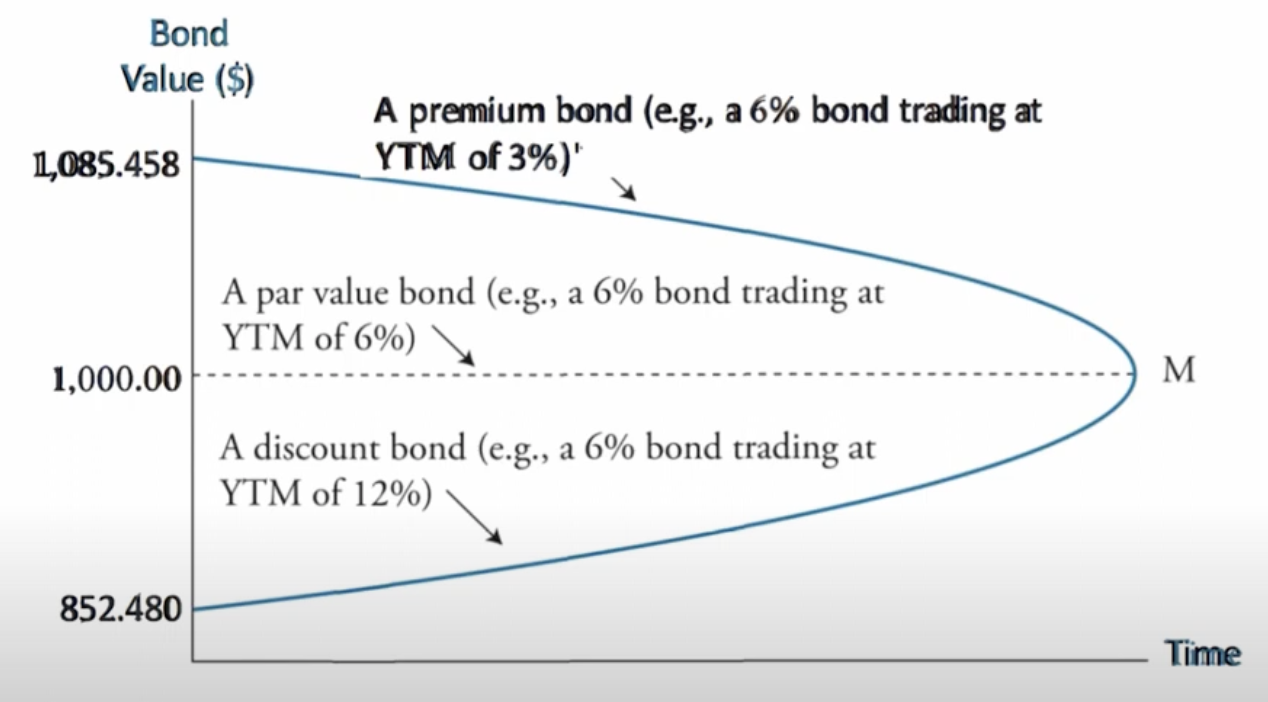
\includegraphics[width=0.5\textwidth]{bond_curve.png}
\caption{The relationship between YTM, coupon rate and price}
\label{loadings}
\end{figure}
 \section{The limitations of traditional yield measures}
 \begin{itemize}
     \item YTM предполагает что все денежные поступления будут реинвестироваться под ставку YTM и будет удерживаться до погашения
     \item Риск реинвестирования присутсвует в купонах которые могут быть реинвестированы под более низкую ставку (это также применимо к досрочно погашенным облигациям и амортизирующим облигациям)
     \item Риск реинвестирования становится более существенной проблемой для более долгосрочных облигаций и облигаций с более крупными купонами
 \end{itemize}
 \section{Coupon effect}
 Облигации с низкой купонной доходностью более чувствительны к изменениям процентных ставок
 \begin{figure}[h]
\centering
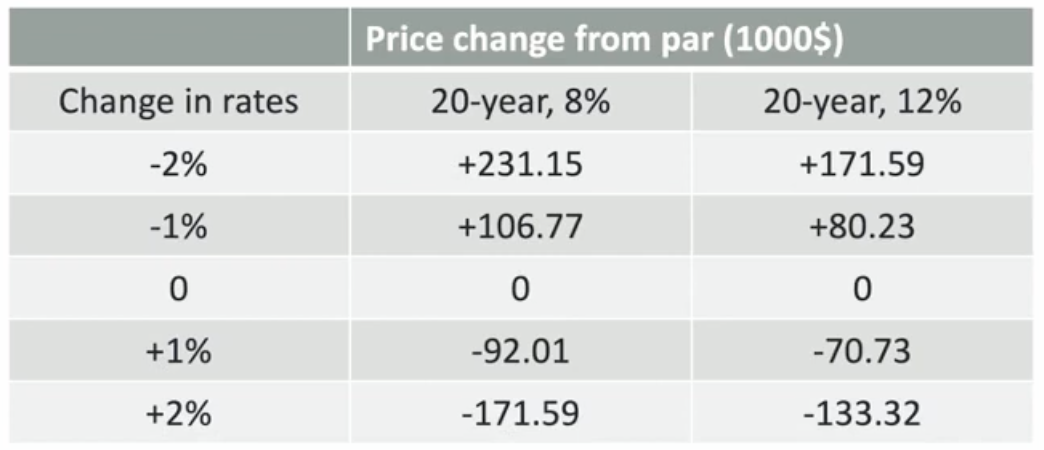
\includegraphics[width=0.5\textwidth]{coupon.png}
\caption{Coupon effect}
\label{loadings}
\end{figure}
\section{Carry roll-down scenarios}
\textbf{Первый сценарий} Carry roll-down создан для расчета доходности полученной в случае если ставка остается неизменной\\

\textbf{Realized forward сценарий:}
 \begin{itemize}
     \item Наиболее частоиспользуемые предпосылки
     \item Форвардная ставка для будущих периодов остается неизменной с течением времени
     \item Когда начинается фьючерсный период, спот ставка для периода равна форвардной ставке
     \item Нет разницы между короткосрочными и долгосрочными инвестициями
 \end{itemize}
\underline{Пример:}\\
Двухгодовая облигация, купон 2.5\%, цена в нулевой момент времени:
 \begin{multline*}
    \frac{1.25}{1 + 0.0035} + \frac{1.25}{(1 + 0.0035)(1 + 0.006)} + \frac{1.25}{(1 + 0.0035)(1 + 0.006)(1 + 0.008)} + \\ \frac{1.25 + 100}{(1 + 0.0035)(1 + 0.006)(1 + 0.008)(1 + 0.01)} = 102.226
\end{multline*}\\
Через 6 месяцев цена будет:
\begin{align*}
    & \frac{1.25}{1 + 0.006} + \frac{1.25}{(1 + 0.006)(1 + 0.008)} + \frac{1.25 + 100}{(1 + 0.006)(1 + 0.008)(1 + 0.01)} = 101.334
\end{align*}\\
За эти 6 месяцев:
 \begin{align*}
    \text{купон} & = 1.25 \text{ у.е.}\\
    \text{изменение цены}  & = 101.334 - 102.226\\
    \textbf{Carry roll-down} & = \textbf{1.25 - 0.892 = 0.358}
\end{align*}
\textbf{Упрощенное вычисление для realized forward scenario: 102.226 * 0.0035 = 0.358}
 \begin{figure}[h]
\centering
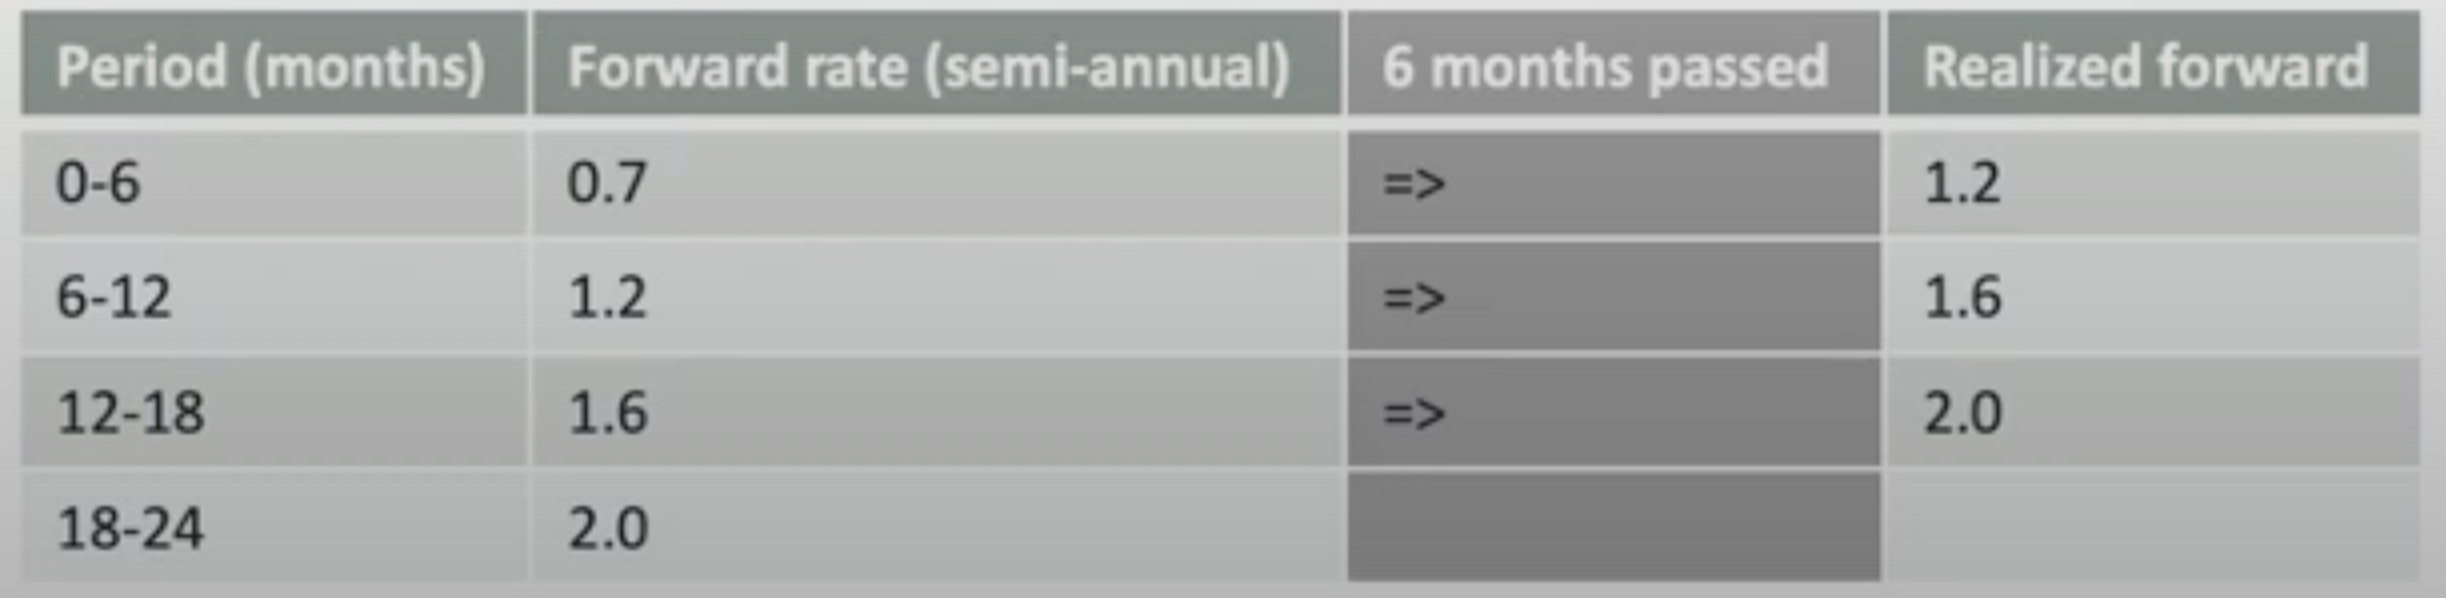
\includegraphics[width=0.6\textwidth]{first.png}
\caption{Первый Carry roll-down сценарий}
\label{loadings}
\end{figure}\\
\textbf{Второй сценарий: когда форвардные ставки при сдвиге во времени не изменяются}. Такое происходит, когда рынок закладывают дополнительную премию за инвестиции на длинные сроки, соотвественно кривая не меняет форму.
 \begin{figure}[h]
\centering
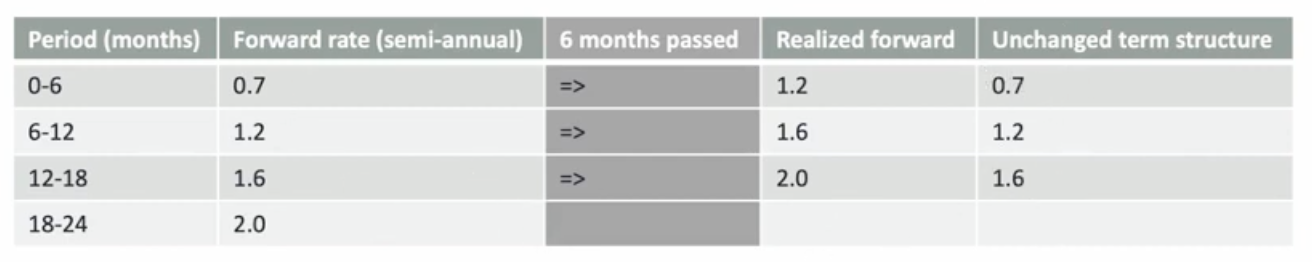
\includegraphics[width=0.8\textwidth]{unchanged.png}
\caption{Второй Carry roll-down сценарий}
\label{loadings}
\end{figure}\\
\textbf{Третий сценарий: Unchanched yields}. В нем предполагается, что доходности облигаций в течение времени не меняются вообще. В таком случае требуется, чтобы купоны реинвестировались по ставке YTM
\section{Return decomposition}
Мы можем разбить \textbf{доходность облигации (Profit and loss, P&L)} на несколько компонентов, две крупные группы этих компонентов это изменение цены и внешний денежный поток (стоимость финансирования и купоны):

\textbf{Изменение цены}
\begin{itemize}
     \item \textbf{Carry-roll-down} изменение стоимости облигации по мере изменение структуры ставок со временем
     \item \textbf{rate changes} скачки в ставках, отличающиеся от нормального изменения ставок со временем
     \item \textbf{spread changes} изменения в спреде, т.е. в надбавке к ставке дисконтирования денежных потоков по облигации
 \end{itemize}
\begin{align*}
    & BV_{t}(R_{t}, S_{t}) - BV_{t-1}(R_{t-1}, S_{t-1}) = \\
    & BV_{t}(R_{t}, S_{t}) - BV_{t}(R_{t}, S_{t-1}) \text{ spread change}\\
    & BV_{t}(R_{t}, S_{t-1}) - BV_{t}(R'_{t}, S_{t-1}) \text{ rate changes}\\
    & BV_{t}(R'_{t}, S_{t-1}) - BV_{t-1}(R_{t-1}, S_{t-1}) \text{ carry-roll-down}\\
\end{align*}
\end{document}
